\documentclass{standalone}
\usepackage{tikz,calc}
\usepackage{amsmath}
\renewcommand{\familydefault}{\sfdefault}


\begin{document}

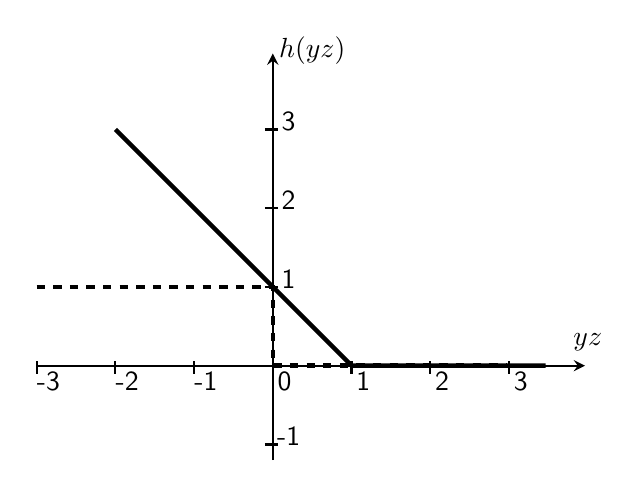
\begin{tikzpicture}[shorten >=1pt,draw=black,thick, node distance=\layersep, >= stealth]

    \draw [->](-3, 0)  --  (4, 0);
    \draw [->](0, -1.2)  --  (0, 4);
    \draw [black, ultra thick, dashed] (-3, 1)  --  (0, 1)  --  (0, 0)  --  (3, 0);

    \draw [black, ultra thick] (-2, 3)  --  (1, 0)  --  (3.5, 0);
    \foreach \x in {-3, -2, -1, 0, 1, 2, 3}{
        \node at (\x + .15, -.2) {\x};
        \draw (\x, -.1)  --  (\x, .1);
    }

    \foreach \y in {-1, 1, 2, 3}{
        \node at (.2, \y + .1) {\y};
        \draw (-.1, \y)  --  (.1, \y);
    }
    \node at (4, .3) {$yz$};
    \node at (.5, 4) {$h(yz)$};
\end{tikzpicture}
% End of code
\end{document}
